\chapter{Approach}
\label{chap:approach}


\section{Mining}

% TODO ensure this is accurate.dfdsf
\gls{oss} generally is software that is provided with the ability access the source code and make modifications to the source code. While certain licenses provide some restrictions on the ability to redistribute the software the main point of the source code of the software being freely available is key. The scope and capability of \gls{oss} projects vary greatly. Several very popular \gls{oss} projects are listed in table \ref{tab:oss_projects}.

%TODO make sure footnotes fit in better.
\begin{table}[h!]
\begin{minipage}{\textwidth} 
\begin{center}
    \begin{tabular}{|l|l|l|}
        \hline
        Owner & Project & Description \\
        \hline

        Mozilla & Firefox\footnote{\url{https://www.mozilla.org/en-US/firefox/desktop/}} & Internet Browser \\
        Linux & Linux Kernel\footnote{\url{https://www.kernel.org/}} & Operation System Kernel \\
        VideoLAN & VLC\footnote{\url{http://www.videolan.org/vlc/index.html}} & Media Player \\
        PostgreSQL & PostgreSQL\footnote{\url{http://www.postgresql.org/}} & Object-Relational Database Management System \\
        git & git\footnote{\url{https://git-scm.com/}} & Version Control System \\
        \hline
    \end{tabular}
\end{center}
\caption{Open Source Software Projects}
\label{tab:oss_projects}
\end{minipage}
\end{table}
%Firefox => MPL 2.0
%Linux Kernel => GPL v2, plus various closed-source binary blobs
%VLC => GPLv2+ (player), LGPLv2.1+ (engine)
%PostgreSQL => PostgreSQL License
%git => GNU General Public License v2, GNU Lesser General Public License 2.1

The development of large software projects (whether \gls{oss} or not) have often made use of \gls{vcs}. A \gls{vcs} helps the developers of the project manage the changes of the project and facilitate the collaboration between developers. A \gls{vcs} will keep an current version of the project and keep track of the previous version of the project as well. This may be done through keeping a copy of each version of the project or by keeping track of all each change made to the project. \gls{svn} and git would be two examples of \gls{vcs}s.

Git is a \gls{dvcs} and differs greatly from \gls{svn} which is a normal \gls{vcs}. Git will provide the user with a complete copy of the repository to be that can be worked on independent of network connection and thus also without a centralized server. The distributed aspect of git allows for easier use for all involved parities. The one main issue with a \gls{dvcs} is that the users will require a means to communicate to transfer changes made to the repository. Therefore typically one centralized server is used to maintain communication between all interested parties.

Git has grown in popularity since it was created and is at the core of several \gls{vcm} sites such as GitHub \footnote{\url{https://github.com/}}, BitBucket \footnote{\url{https://bitbucket.org/}} and GitLab \footnote{\url{https://gitlab.com/}}. These platforms tend to be fairly supportive of \gls{oss} projects through providing their services free of charge. For example, GitHub provides unlimited public repositories completely free. While these projects do not have to be licensed with an open source license typically they will be since they are already publicly visible.

% GitLab -> https://gitlab.com/
% GitHub -> https://github.com/
% BitBucket -> https://bitbucket.org/

GitHub is the most popular of the \gls{vcm} websites and hosts numerous very popular \gls{oss} projects including, the Linus Kernel, Swift\footnote{\url{https://swift.org/}} and React\footnote{\url{https://facebook.github.io/react/}}. GitHub also provides a public \gls{api} to allow for access to the data related to project repositories which is discussed further below. % TODO link to that.
Given the popularity of GitHub for use by developers and the availability of the project data, GitHub is a obvious choice for mining project data. Especially since the target for mining software was to capture \gls{oss} projects to for testing. Publicly visible projects are also publicly accessible through the \gls{api} and the majority are open source.

%%%%%%%%%%

Git provides a simple interface to manage the repository regardless of which site is the central server. Therefore regardless which site the project resides on users can easily interact with the project as long as they know the git interface. Git in essences is a file storage for the project that keeps track of changes made to the project. A \textit{commit} is a set of changes that a developer has made at a certain time. The developer has full control what gets committed, when it gets committed and even modified at a later date. Therefore the date of the commit merely means when the developer notified Git that a change was made.

A branch is a series of commits that are often related. In figure \ref{fig:network_diagram}, each dot would represent a commit and a set of dots connected by the same colored lines are a branch. Branches can be considered different paths or deviations in the development from each other allowing for different versions of the project to be maintained and developed. The \textit{master} branch is the main branch, represented with black, from which all branches usually stem from and is generally where projects are developed on. On a similar note, a \textit{tag} is a branch that is frozen to allow for future reference. Often tags are uses to mark a significant point in the development history such as a project release. Finally, when two differently branches converge into a single dot then the two branches have been \textit{merged}. A merge indicates that the differences between the two branches are consolidated based on the developer's discretion.

\begin{figure}[!ht]
    \centering
        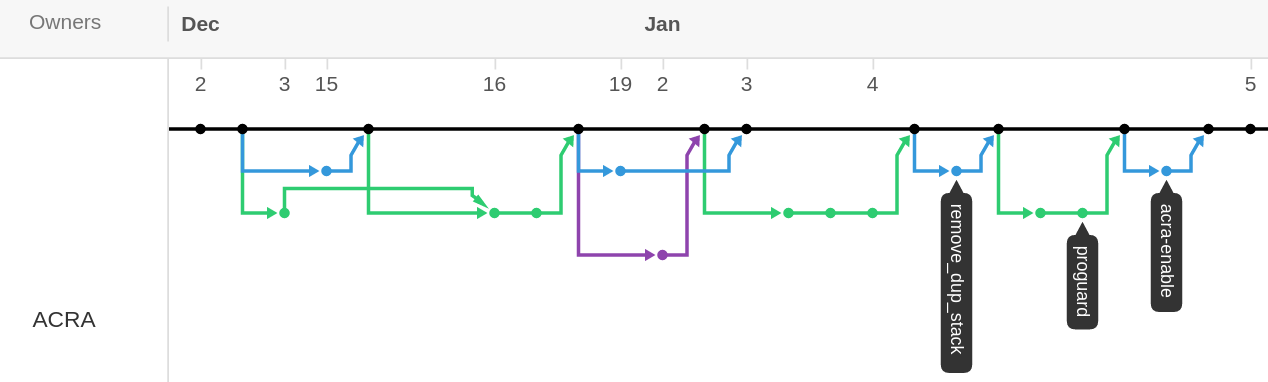
\includegraphics[width=1.0\textwidth]{images/network}
    \caption{Network diagrams}
    \label{fig:network_diagram}
\end{figure}

A commit consists of files that have been changed, more specifically a list of \textit{patch} files which each outline the changes made to their corresponding file. The patch file consists of a series of differences between the previous version of the file and this new version of the file. These patch files are key since they contain the actual changes made to the project and thus are the major point of interest.

In order to be able to predict changes within a project some project data must first be collected. The data collection is targeted towards open source projects that use GitHub. Specifically projects that are predominately written in Java. The overall method is not language specific however for the purpose of simplifying the implementation it was restricted to only allow for Java. The data collection simply collects all the project's development history realized through the changes made to the project. This includes the information related to developers, commits, tags (releases) and files in the project.

The data is kept unprocessed and stored directly into a relational database (MySQL) which allows the data to be used and manipulated without requiring access to GitHub again. This was ideal during the more initial phase of the research allowing for various methods of analysis to be applied on the data set without requiring the data to be download again. The collection of data can take long to perform and depends largely on the size of the project. The collection process also allows for a partial collection of newly added project changes after the initial collection of the project. This allows for the changes made to the project after the initial collection of project data to be collected as well. These maintenance collections will often be much smaller and require a smaller amount of time to collect.


%<<< TODO create a table which outlines the data elements >>>
% TODO create a figure of an api return

The method chosen for collecting data for GitHub projects was using GitHub's web \gls{api}. The GitHub \gls{api} allows for access to the complete set of publicly available information stored in GitHub. Accessing the data through the \gls{api} allows for the process to be automated and vastly simplifies the process. This data set can be rather large since it includes a snapshot of the commit, all the change data and developer data related. In order to collect data the repository name and the name of the user who owns the repository must be known.

% TODO talk about the collection script - how it takes a project, collects all the commits and then goes commit by commit extracting the necessary 

% TODO integrate this with above explanation of VCS and git
Some aspects of the GitHub project's data set are not collected as they were deemed unnecessary however it could easily be extended to collect the other aspects. The aspects not collected are the issues, branches, forks and pull requests. The issues data outlines the problems reported in the project by users or developers of that project. GitHub allows for issues to be optional and thus some projects do not offer issue reporting through GitHub. Branches are also directly related to the project and they are essentially different workspaces for the developers. They allow for development of different versions (such as a development version compared to a stable version). The simplicities sake this project assumes that the main branch (master) is the development branch and the target of the analysis. Of course other branches could be analyzed however the perspective of the other branches typically originates from the master branch.

A similar sub-data set not collected or used is forks of the repository. For GitHub a fork is an externally created branch. This allows for a developer who does not own the project (but can view it) make a copy of the project and work on it without affecting the original. Forks differ slightly from branches in that they typically denote a deviation from the original project that is unlikely to be reconciled. Finally, pull requests facilitate external developers making small changes and are typically fixes to found problems or desired feature implementation. The owner of the repository can then decide to integrate the changes made the original repository.


%- TODO explain a little more
%    - about using the api commands and how this is entirely automatic. Simply point to repo owner and name and it collects
%    - language agnostic for collection
%    - What is not collected:
%        - issues
%        - forks
%        - pull requests

\section{Storage}

As mentioned above the data is stored in a MySQL relational database which leverages \gls{sql}. There are two databases used for the collection and the analysis. One stores the raw mined data, whereas the second stores the analyzed data in a more convenient layout to be used later. A third database was later added for the change prediction and uses a different relational database implementation because of some limitations within MySQL. This third database uses PostgreSQL, which has some more advanced features than MySQL and is simply a clone of the second database. The specific limitations that were encountered will be discussed more fully later on in this section.

% TODO add a figure of the database schema.

%TODO re-factor this
The first database called \textit{github\_data} and stores the semi-raw data collected from GitHub's \gls{api}. This database contains 8 tables which store various aspects about the projects that were considered potentially important for the analysis later on. The tables of primary concern are \textit{repositories}, \textit{commits}, \textit{users}, \textit{files} and \textit{tags} tables. While not all of the data available from GitHub's \gls{api} is collected primary aspects are and the database could be extended to store more of the dataset if necessary. The only real difference between the raw data and the data stored in the \textit{github\_data} database is a slight layout changes and removing invalid or inaccessible data.

After storing the data in the \textit{github\_data} database, the analysis process is done. The \textit{parsing} script is run next and discussed further in the section \ref{sec:parsing}. This database, \textit{project\_stats}, is very similar in layout to the first database some extra tables have been added and a few data items have been removed. Mostly the storage expansions have been to hold change information calculated from the analysis of the data.

The final database uses PostgreSQL because of limitations within the MySQL implementation. Some of the candidate features discussed in more detail in section \ref{sec:sample_data} required a more versatile partitioning function and the ability to perform multiple inner queries. The first of which is more difficult to implement and the second is not available at all MySQL.

In order to transfer the data over to PostgreSQL a simple program called \textit{pgloader} was used to transfer the MySQL database over to PostgreSQL. Only one difficulty was encountered during the transferring process. One of the tables in the MySQL database was called \textit{user}, however in PostgreSQL this is a reserved table name and therefore the table cannot be interacted with properly. The work around was to simply rename the table in MySQL prior to transferring to avoid any issues with the database. Once the database is copied over to PostgreSQL it is ready to be used for to perform change prediction.

\section{Parsing}
\label{sec:parsing}

When the data has been collected and stored it can then be analyzed to extract more refined details. The changes made per commit can be analyzed to extract the number of methods added, deleted and modified per commit. The process first requires the changes from a commit, the patches, to be merged into their corresponding full file. A patch is simply a summarized stub of the full file which allows for a quick reference as to which line is changed and what change occurred on that line. The three different types of changes that can appear within a file are deletions, additions and no change. These are represented as a minus sign, plus sign and space respective.

% TODO talk about these different changes
% TODO consider getting different images (for removed, changed, and unchanged) all of them are too wide and the scaling looks terrible.
% - Fix by zooming in and then refreshing the page, make sure to get a piece of code that is not to wide.
\begin{figure}[!ht]
    \centering
        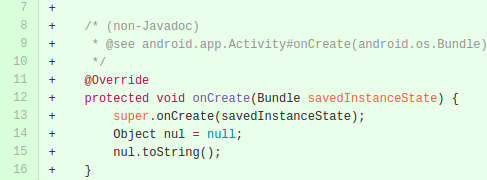
\includegraphics[width=0.80\textwidth]{images/added_example}
    \caption{Newly added method}
    \label{fig:added_method}
\end{figure}

\begin{figure}[!ht]
    \centering
        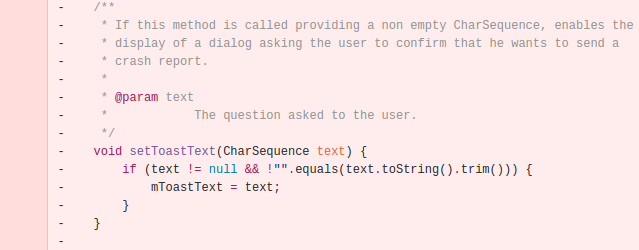
\includegraphics[width=0.80\textwidth]{images/deleted_method}
    \caption{Removed method}
    \label{fig:removed_method}
\end{figure}

\begin{figure}[!ht]
    \centering
        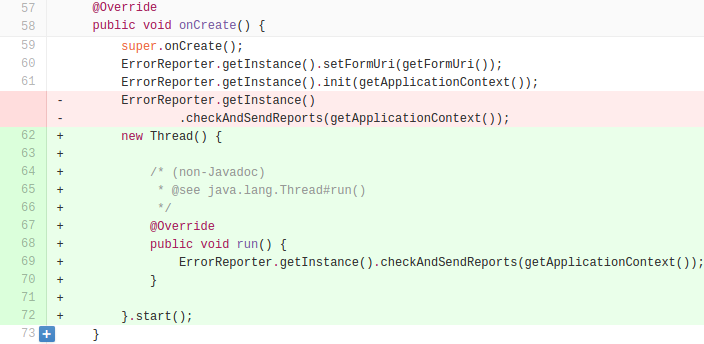
\includegraphics[width=0.80\textwidth]{images/simple_complex}
    \caption{Mixed changed method}
    \label{fig:changed_method}
\end{figure}

\begin{figure}[!ht]
    \centering
        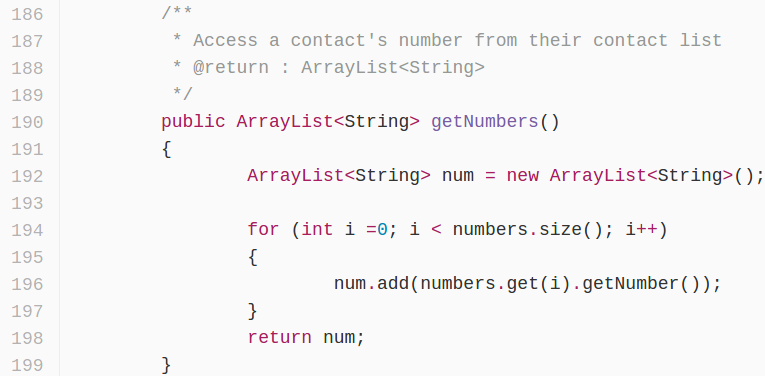
\includegraphics[width=0.80\textwidth]{images/unchanged_example}
    \caption{Unchanged method}
    \label{fig:unchanged_method}
\end{figure}


Using the patch file a \textit{deleted} file can be reconstructed by removing all lines marked as added from the file and adding the lines marked as deleted back into their original location. This allows for both added and deleted methods to be identified by using the original file for detecting the location of added methods and the \textit{deleted} file to detect deleted methods.

%- Note that an added method is one such that every line of code within it is newly added. Likewise a deleted method is one such that every line of code in removed.

The more difficult method to identify is one which has been modified. Again use of the two files will be necessary, in this case we will identify methods from each which are not entirely additions or deletions respectively. The union of these two sets of methods will be taken to determine the number of methods that have been modified. For each commit this information is stored to allow for easier access and save time since the analysis of larger data sets can be time intensive. In order to maintain the integrity of the initial data set this information is stored in a new database.

%- TODO also describe the collection of method line changes

%<<< TODO create a table which outlines the metrics stored >>>

\section{Analysis}
\label{sec:analysis}
% TODO talk even more about how to pick better features.

A \gls{svm} is used to predict what type of change will occur based on a set of features provided. A feature is a data extracted from the project represented as a floating point number. In order to be useful a feature must in some way characterize the the category that it is assigned to. The feature must also not rely on the category that it belongs to in order to be calculated. For example, if the category is whether the project will change in the future or not, then the features must not rely on knowledge of future changes to the project. If the features fail to effectively characterize the category they are assigned to then the \gls{svm} may have poor predictions. It is also necessary for the featur  es to independent of each other to not negatively affect the categorization.

%<<< TODO Example feature vector >>>

% \begin{table}
% \begin{center}
%     \begin{tabular}{|l l l l l l l|l|}
%         \hline
        
%         Features &  &  &  &  &  &  & Description \\
%         \hline
%         $name$ & $signature$ & $change_i$ & $committer$ & $freq_{change}$ & $change_{prev}$ & $t_\Delta$ & $change_{next\_6}$ \\
%         %0.0 & 0.1 & 0.0\\
%         \hline
%     \end{tabular}
% \end{center}
% \caption{Example Feature Vector}
% \label{tab:example_feature_vector}
% \end{table}

% TODO Format parts of this.
\gls{svm} requires all feature data be encoded as floating point numbers. For any numerical data the conversion to floating point is trivial. However, for more complex data the conversion is a little more difficult. Categorical data can be mapped into a unique vector entry per category. For example, if a feature can be 1 of 3 options: 0, 1 or 2 then it can be converted into three entries in the feature vector. Encoding the value 2 the sub-vector of the feature set would be [0, 0, 1] where 1 indicates a field that feature is present in the data for this vector, and 0 indicates the feature is not present. Data that is in the form of a string can be converted to a floating point number by assigning a unique number for each string (similar to hashing). The one downside to this method is that the numbers corresponding to each string maintain no numerical properties. In essence the data becomes categorical, such that if \'bob\' is mapped to 1 and \'sally\' is mapped to 2 there is no relationship between 1 and 2. Ideally, this data would then be further converted using the previously described method however if the set of possible strings is large than it may be unreasonable to convert it. For example, if there are 100 possible strings then that would add 100 new entries to a single vector.

%<<< TODO svm diagrams >>>

The categorization is used for the prediction, where each value of the category relates to a unique prediction type. For example, a simple binary categorization could simply 1 or 0 where 1 predicts the event will occur and 0 predicts that the event will not occur. In essence an \gls{svm} is tasked with separating a data set that has be categorized into 2 subsets. Once the data set has been separated new data can be provided that has not be categorized to allow for the \gls{svm} to predict which category the new data vector belongs too. More specifically a sample data set is extracted from the target data set. It is then categorized based on the predetermined criteria. This data set along with the categorization for each vector in the data set is the training data set, and is then used to \textit{train} the \gls{svm} model. Once the model has been trained, the \gls{svm} model is ready to be used. The data for each features can be extracted from the new dataset, allowing for the model to classify each new vector. Once classified the developer can take the appropriate course of action. For example if the classification is that of predicting change to occur within the next six commits the developer may wish to be careful with the use of the method or assess the method's quality and determine if any issues within the method need to be addressed.

A lower prediction score often relates to the data from the feature set poorly characterizing the categories. Similarly a warning will be given if the data set is in-separate. In this case, the data set for each category may be too similar and cannot be properly split into the two category subsets. In both cases a change to the feature set may help, whether that is a decrease or increase of features in the set. Some features are detrimental to the model, especially if these features are in some way related to another feature. Other potential steps would be to modify the data to ...
% *** TODO determine best practices for data something like mean of 1 and std of 1. ***

More detail about the specific features used will be given a little later on. Features are descriptive aspects of the data set that are classified into the predetermined categories. Since these features relate directly to the category that they are helping describe any feature must first know what the classification is. For example for a classification of whether a change will occur within the next few commits, a useful feature may be the frequency by which a methods changes within the project. Picking a descriptive feature set is paramount to providing a strong prediction of future data.

%<<< TODO create a figure to outline the various features and their meaning >>>

Most of this was done using database queries or user defined functions created in the database language.